\section{Smooth approximation}
\label{sec:smooth apx}
\newcommand{\fe}{f_\varepsilon}

\subsection{The need for smoothing}
\label{sec:need for smoothing}
Let $\formula$ be an MTL formula with horizon $N$.
We aim to solve the following control problem $P_\rob$.
\begin{subequations}
\label{eq:general_ctrl}
\begin{align}
P_\rob:\, \max\, & \rob_{\formula}(\sstraj) - \gamma \sum_{k=0}^{N-1} l(x_{k+1},u_{k}) \label{eq:general ctrl obj}\\
\text{s.t. } & x_{k+1} = f(x_k,u_k), \, \forall k=0,\dotsc,N-1 \label{eq:general ctrl dyn}\\
 & x_k \in X, \, \forall k=0,\dotsc,N \label{eq:general ctrl X}\\
 & u_k \in U, \, \forall k=0,\dotsc,N-1 \label{eq:general ctrl U}\\
 & \delta \rob_{\formula}(\sstraj) \geq 0 \label{eq:general ctrl pos rob}
\end{align}
\end{subequations}

We want to use established, powerful gradient descent algorithms \cite{Polak97_Optim}, rather than heuristics like Simulated Annealing \cite{kirkpatrickV_SA83}. 
In the above formulation, $l(x_{k+1},u_{k})$ is a system specific control cost, e.g. the LQR cost $x_k'Qx_k + u_k'Ru_k$. $\gamma \geq 0$ is weighting parameter, which is a design choice. $X$ and $U$ define constraints on the state $x$ and control $u$ respectively. $f$ represents the dynamical system, with $x$ as the state and $u$ as inputs. Finally, the last constraint enforces $\rob \geq 0$, i.e. the specification is satisfied. 
$\delta$ here is a binary design choice, $1$ if the constraint is meant to be enforced, $0$ otherwise.
We will need to assume that $f$ is twice Lipschitz continuously differentiable and that its gradient $f_u$ has maximum row rank.

Gradient descent algorithms typically offer convergence guarantees to the function's minima, have known convergence rates for certain function classes, and have been optimized so they outperform heuristics that don't have access to the objective's gradient information.
Moreover, they usually have a fewer number of parameters to be set by the user, and important issues like step-size selection are rigorously addressed.

To apply gradient descent methods, we require a differentiable objective function. 
Our objective function, $\robf$, is non-differentiable, because it uses the distance, max, and min functions, all of which are non-differentiable.
One may note that these functions are all differentiable almost everywhere (a.e.).
That is, the set of points in their domain where they are non-differentiable has measure 0 in $\Re^n$. 
Therefore, by measure additivity, the composite function $\robf$ is itself differentiable almost everywhere.
Thus, one may be tempted to `ignore' the singularities (points of non-differentiability), and apply gradient descent to $\robf$ anyway.
The rationale for doing so is that sets of measure 0 are unlikely to be visited by gradient descent, and thus don't matter. 
However, as we show in the next example, the lines of singularity (along which the objective is non-differentiable) can be  precisely the lines along which the objective increases the fastest.
See also \cite{Cortes08_Discontinuous}.
Thus they are consistently visited by gradient descent, after which it fails to converge because of the lack of a gradient.


\begin{exmp}
	\label{ex:cluster nondiff}
	A simple example illustrates how gradient descent gets stuck at singularities.
	We use Sequential Quadratic Programming (SQP) \cite{Polak97_Optim} to maximize the robustness of $\formula = \neg (x \in U)$, where $U=[-1,1]^2$ is the unsafe red square in Fig.~\ref{fig:DumbExample}.
	In this case, $\robf$ is simply $\dist(x_0,U)$, the distance of the first trajectory point to the set.
	The search space is $[-2.5,2.5]^2$ (big grey square in Fig. \ref{fig:DumbExample}). 
	The most robust point is $x^* = [2.5,2.5]$ (green `+' in figure), being furthest from the unsafe set.
	We initialize the SQP at $x_0=[0,0]$. 
	SQP generates iterates (blue circles) \textit{on the line of singularity} connecting $[1,1]$ to $x^*$ and ultimately gets stuck at $x=[1,1]$.
	That's because along the line, the gradient does not exist and attempts by SQP to approximate it numerically fail, prompting it to generate smaller and smaller step-sizes for the approximation.
	Ultimately, SQP aborts due to the step-size being too small, and concludes it is at a local minimum.
	
\begin{figure}[t]
\centering
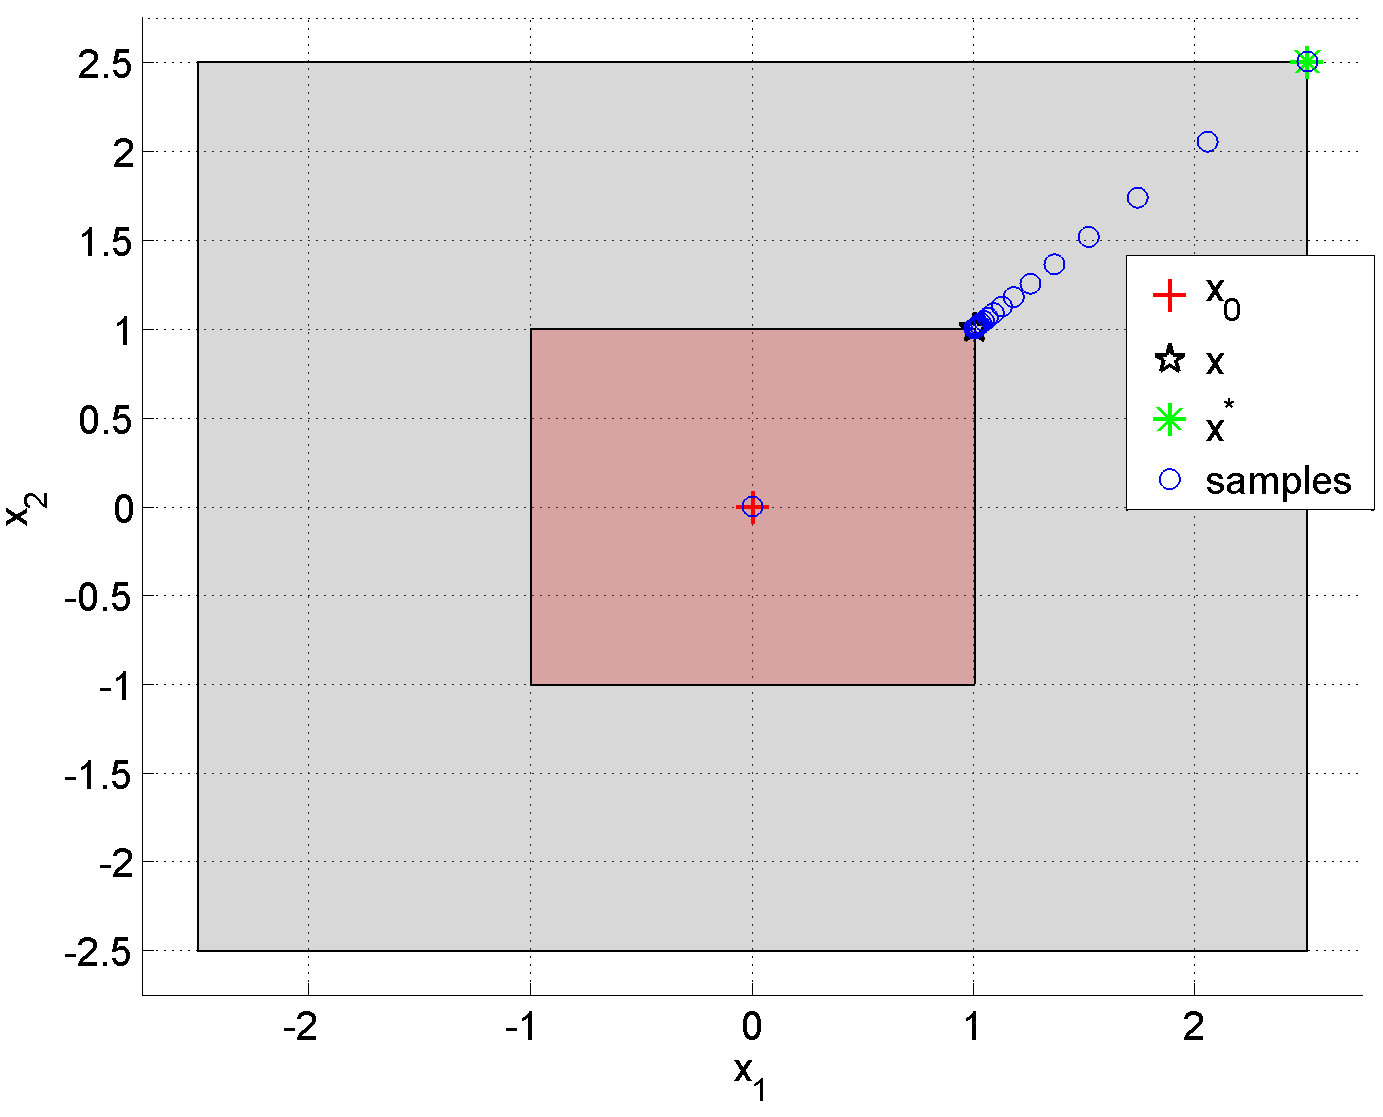
\includegraphics[width=0.49\textwidth]{figures/DumbOptEx_scissored}
\vspace{-20pt}
\caption{{\small Iterates of SQP for Example \ref{ex:cluster nondiff}. Colors in online version.}}
\vspace{-10pt}
\label{fig:DumbExample}
\end{figure}

\end{exmp}

\subsection{Approximating the distance function}
\label{sec:dist smoothing}
To create a smooth approximation to $\robf$, we use smooth approximations to each of its non-differentiable components: the set-distance, min, and max functions.

\begin{figure}[t!]
	\centering
	\begin{subfigure}[t]{0.25\textwidth}
		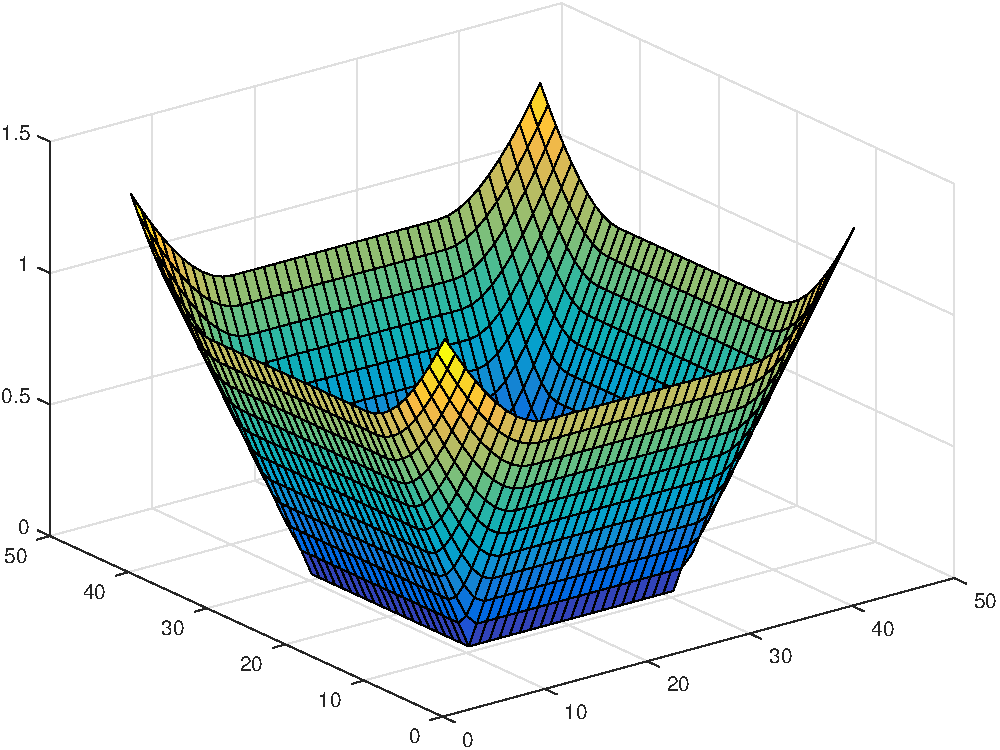
\includegraphics[height=1.2in]{figures/smoothDist2d}
		\caption{Smoothed function}
	\end{subfigure}%
	~
	\begin{subfigure}[t]{0.25\textwidth}
		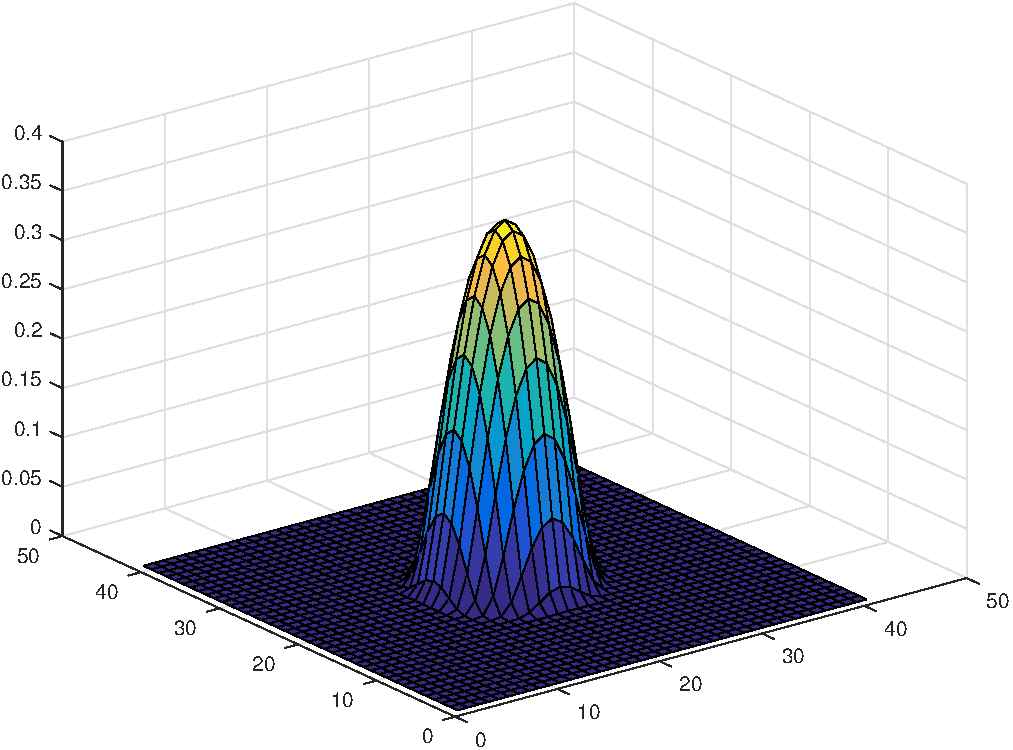
\includegraphics[height=1.2in]{figures/kernelG}
		\caption{Function $g$}
	\end{subfigure}
	\caption{{\small Smoothed 2-d distance function to a square in the x-y plane, and the function $g$ used to smoothen it.}}
	\vspace{-20pt}
	\label{fig:smooth2d}
\end{figure}

Recall that for a set $U \subset \Re^n$, $\dist(x,U) = \inf_{a \in \cl{U}} |x-a|_2$, where $|\cdot|_2$ is the Euclidian norm.
This function is globally Lipschitz with Lipschitz constant 1 and therefore differentiable almost everywhere (Rademacher's theorem), and has a second derivative almost everywhere if $U$ is convex (Alexandrov's theorem) \cite{MakelaN92book}.

It is well-known that if we convolve an a.e.-differentiable function with a smooth kernel, the output function no longer has those singularities.
We give an example of such a construction, which lays the groundwork for explaining the more general wavelet-based smoothing we use in the experiments.
$C^\infty(\Re^n)$ is the class of functions that are infinitely differentiable in $\Re^n$.
\begin{theorem}
	\label{thm:ge smoothing}
	Consider the globally Lipschitz function $f:\Re^n \rightarrow \Re$ with Lipschitz constant $L_f$.
	Let $g: \Re^n \rightarrow \Re_+$ be a non-negative $C^\infty(\Re^n)$ function that integrates to 1 and is supported on the unit ball:
	$\int_{\Re^n}g(x)dx = 1$, $g(x) = 0$ if $x \notin B(0,1)$.
	Define $g_\varepsilon = \varepsilon^{-n}g(x/\varepsilon)$ and
	\[f_\varepsilon(x) = f *g_\varepsilon(x) = \int_{\Re^n}f(y)g_\varepsilon(x-y)dy\]
	Then $\fe$ is infinitely differentiable, its Lipschitz constant $L_{\fe} \leq L_f$ and $\|f-\fe\|_\infty \leq L_f \varepsilon$.
\end{theorem}
\begin{proof}
	Clearly, $\fe$ is $C^\infty$: $g_\varepsilon \in C^\infty$ and the integrand in the above convolution is differentiable w.r.t. $x$, so it holds that $\fe'(x) = \int{f(y)\partial g_\varepsilon(x-y)/\partial x dy}$.
	
	Convolution is commutative so $f_\varepsilon(x) = \int_{\Re^n}f(x-y)g_\varepsilon(y)dy$.
	Let $x' \in \Re^n$, then 
	\begin{eqnarray*}
	|\fe(x)-\fe(x')| &=& |\int_{\Re^n} f(x-y)g_\varepsilon(y) - f(x'-y)g_\varepsilon(y) dy|
	\\
	&\leq & \int_{\Re^n} g_\varepsilon(y)|f(x-y) - f(x'-y)| dy
	\\
	& = & L_f|x-x'| \int_{\Re^n} \varepsilon^{-n} g(y/\varepsilon) dy
	\\
	&= &L_f|x-x'| \int_{\Re^n} \varepsilon^{-n} g(y') \varepsilon^ndy'
	\\
	&=& L_f|x-x'| \implies L_f \leq L_{\fe}
	\end{eqnarray*}
	
	Finally, 
	\begin{eqnarray*}
	|\fe(x)-f(x)| &=& \left|\int_{\Re^n}f(x-y)g_\varepsilon(y)dy - \int_{\Re^n}f(x)g(y)dy\right|
	\\
	&=& \left|\int_{\Re^n}f(x-\varepsilon y)g(y)dy - \int_{\Re^n}f(x)g(y)dy\right|
	\\
	&\leq& \int_{B(0,1)}|f(x- \varepsilon y) - f(x)|g(y)dy	
	\\
	&\leq & \int_{B(0,1)}L_f | \varepsilon y| g(y)dy \leq L_f \varepsilon
	\end{eqnarray*}
	In particular, $\|f-\fe\|_\infty \rightarrow 0$ as $\varepsilon \rightarrow 0$.
\end{proof}
Fig.~\ref{fig:smooth2d} shows the distance function $\dist(\cdot,U)$ where $U$ is a square in the plane, smoothed by convolving with kernel $g_{\varepsilon}$ obtained from the shown function. 
We used $\varepsilon = 0.001$, and the actual approximation error $\|f-\fe\|_\infty$ is less than 1e-15.
Parameter $\varepsilon$ controls how peaked or flat $g_\varepsilon$ is: a large $\varepsilon$ gives a peaked kernel which yields better local approximation, but the max error decreases towards 0 slower.

%\todo[inline]{because lip cnt is bounded by that of f, this says that it's a conservative apx? if d is -ve and decreasing, $d_\varepsilon$ decreases less and if d is +ve and increasing, $d_e$ increases less.}

\subsection{Wavelet approximations}
\label{sec:waveletApx}

Wavelets can be viewed as a generalization of the kernel $g_\varepsilon$ of the previous section to a whole family of kernels, obtained by translations and dilations of one function called the `mother wavelet' $\psi$: $\psi_{k,j}(x) = \sqrt{2^{-j}}\psi(2^{-j}(x-k))$  \cite{MallatBook}.
They are used extensively in signal processing, as they have very good approximation properties, including fast convergence and multi-scale analysis.
See \cite{MallatBook}.
In the experiments in the rest of this paper, we used the Meyer wavelets. 
Specifically
\todo[inline]{Yash, meyer}
 

\subsection{Smooth max and min}
\label{max min smoothing}
We use the following standard smooth approximations of $m$-ary max and min.
Let $k \geq 1$.
\begin{eqnarray}
	\label{eq:soft max min}
	\smax_k(a_1,\ldots,a_m) &\defeq& \frac{1}{k} \ln(e^{ka_1}+\ldots+e^{ka_m})
	\\
	\smin_k(a_1,\ldots,a_m) &\defeq& -\smax(-a_1,\ldots,-a_m)
\end{eqnarray}
Suppose $k=1$ and that $a_1$ is the largest number.
Then $e^{a_1}$ is even larger than the other $e^{a_i}$'s, and dominates the sum. 
Thus $\smax_1(\mathbf{a}) \approxeq \ln e^{a_1} = a_1 = \max(\mathbf{a})$.
If $a_1$ is not significantly larger than the rest, the sum is not well-approximated by $e^{a_1}$ alone.
To counter this, the scaling factor $k$ is used: it amplifies the differences between the numbers.
It holds that for any set of $m$ reals,
\begin{eqnarray}
\label{eq:smooth max error}
0 \leq \smax_k(a_1,\ldots,a_m) -\max(a_1,\ldots,a_m) \leq \ln(m)/k
\\
0 \leq \min(a_1,\ldots,a_m) -\smin_k(a_1,\ldots,a_m) \leq \ln(m)/k
\end{eqnarray}
Indeed, the error of smooth max can be bounded as follows.
Assume $a_1$ is the largest number, then 
\begin{eqnarray*}
\varepsilon_M &\defeq& \smax_k(\mathbf{a}) - a_1 =  \frac{\ln(\sum_ie^{ka_i})-ka_1}{k}
\\
&=& k^{-1}\ln\left(\frac{\sum_ie^{ka_i}}{e^{ka_1}}\right) \leq k^{-1}\ln \left(\frac{me^{ka_1}}{e^{ka_1}}\right)
\\
&=&\frac{\ln m}{k}
\end{eqnarray*}
It is also clear from what preceded that $\varepsilon_M \geq 0$.
The maximum error is achieved when all the $a_i$'s are equal.
\subsection{Overall approximation}
\label{sec:overall apx}
Putting the pieces together, we obtain the approximation error for the robustness of any MTL formula.
\begin{theorem}
	\label{thm:total apx error}
	Consider an MTL formula $\formula$ and reals $\varepsilon > 0$ and $k \geq 1$. 
	Define the \textit{smooth robustness} $\srobf$, obtained by substituting $\sdist_{\varepsilon}$ for $\mathbf{dist}$, $\smax_k$ for $\max$, and $\smin_k$ for $\min$, in Def. \ref{def:robustness estimate}.
	Then for any length-$N$ trajectory $\sstraj$, it holds that
	\[|\robf-\srobf| \leq \delta_\formula\]
	where $\delta_\formula$ is
	(a)independent of the evaluation time $t$, and 
	(b) goes to 0 as $\varepsilon \rightarrow 0$ and $k \rightarrow \infty$.
%	\[|\robf-\srobf| \leq |\formula| \cdot \max(\varepsilon,\ln(m)/k)\]
%	where $m$ is the length of the longest temporal interval appearing in $\formula$ and $|\formula|$ is the size of the formula, i.e. the number of operators that appear in it.
\end{theorem}
\begin{proof}
	We will prove a stronger result that implies the theorem.	
%	Define $\delta_\formula \in \Re_+$ inductively: 
%	$\delta_\top = 0, \delta_p = \varepsilon$, $\delta_{\neg \formula} = \delta_\formula$, 
%	$\delta_{\formula_1 \lor \formula_2} = \delta_{\formula_1 \land \formula_2} = \delta_{\formula_1} \sqcup \delta_{\formula_2} + \ln(2)/k$,
%	$\delta_{\formula_1 \until_{[a,b]} \formula_2}  = \delta_{\formula_1} \sqcup \delta_{\formula_2} + \ln(b-a)/k$.
%	Noting that $\delta_\formula \leq |\formula| \cdot \max(\varepsilon,\ln(m)/k)$, it suffices to show that the error is upper-bounded by $\delta_\formula$.
	When $\sstraj$ or $t$ are clear from the context, we will drop them from the notation.
	
	The proof is by structural induction on $\formula$, and works by carefully characterizing the approximation error.
	The case $\formula = \top$ is trivial.
	
\underline{Case $\formula = p \in AP$.}
$\robf(\sstraj,t)$ is given by either $\dist{x_t}{\Oc(p)}$ or $-\dist{x_t}{\Oc(p)}$, and 
$\srobf(\sstraj,t)$ is given by either $\sdist_\varepsilon(x_t,\Oc(p))$ or $-\sdist_\varepsilon(x_t,\Oc(p))$, respectively.
Either way, $|\srobf(\sstraj,t) - \robf(\sstraj,t)| \leq \varepsilon$.
Indeed, $\varepsilon$ satisfies the conditions on $\delta_\formula$.

\underline{Case $\formula = \neg \formula_1$} 
$|\rob_{\neg \formula_1}(\sstraj,t)-\srob_{\neg \formula_1}(\sstraj,t)| = |-\rob_{\formula_1}(\sstraj,t) + \rob_{ \formula_1}(\sstraj,t)|  \leq \delta_{\formula_1}$, and $\delta_{\formula_1}$ satisfies (a)-(b) by induction hypothesis.

\underline{Case $\formula = \formula_1 \lor \formula_2$}.
If the same sub-formula $\formula_i$ achieves the max for both $\rob_{\formula_1}(\sstraj,t) \sqcup \rob_{\formula_2}(\sstraj,t)$ and $\srob_{\formula_1}(\sstraj,t) \sqcup \srob_{\formula_2}(\sstraj,t)$, then by induction hypothesis we immediately obtain 
$|\robf(\sstraj,t)-\srob(\sstraj,t)|  \leq \delta_{\formula_i} \leq \delta_{\formula}$.

Otherwise if, say, $\robf = \rob_{\formula_1}$ and $\srobf = \srob_{\formula_2}$ then
\[\robfa -\delta_{\formula_1} \leq \srob_{\formula_1} \leq \srob_{\formula_2} \implies \robfa-\srob_{\formula_2} \leq \delta_{\formula_1}\]
Also 
\[\srob_{\formula_2} \leq \robfb+\delta_{\formula_2} \leq \robfa + \delta_{\formula_2} \implies -\delta_{\formula_2} \leq \robfa - \srob_{\formula_2}\]
Therefore
\begin{equation*}
\label{eq:inter}
-(\delta_{\formula_1} \sqcup \delta_{\formula_2})\leq \robfa - \srob_{\formula_2}\leq \delta_{\formula_1} \sqcup \delta_{\formula_2} \Leftrightarrow |\robfa - \srob_{\formula_2}|\leq \delta_{\formula_1} \sqcup \delta_{\formula_2}
\end{equation*}
Similarly, if $\robf = \rob_{\formula_2}$ and $\srobf = \srob_{\formula_1}$, we have $|\robfb - \srob_{\formula_1}|\leq  \delta_{\formula_1} \sqcup \delta_{\formula_2}$.
So in all cases, 
\[|\robfa \sqcup \robfb - \srob_{\formula_1} \sqcup \srob_{\formula_2}|\leq \delta_{\formula_1} \sqcup \delta_{\formula_2}\]
Therefore by the triangle inequality and \eqref{eq:smooth max error}
\[|\robfa \sqcup \robfb - \smax_k(\srob_{\formula_1} , \srob_{\formula_2})|\leq  \delta_{\formula_1} \sqcup \delta_{\formula_2} + \ln(2)/k  = \delta_\formula\]
Clearly, $\delta_\formula$ satisfied (a)-(b).

The case $\formula_1 \land \formula_2$ is treated similarly.

\underline{$\formula = \formula_1 \until_I \formula_2$.} 
Before proving this case, we will need the following lemma, which is provable by induction on $n$:
\begin{lemma}
	\label{lemma:n-ary apx}
	If $\formula = \formula_1\land \ldots\land \formula_n$ or $\formula = \formula_1\lor \ldots\lor \formula_n$, $n\geq 2$, then 
	$|\robf - \srobf| \leq \sqcup_{1\leq i \leq n}\delta_{\formula_i} + \ln(n)/k$.
\end{lemma}

We now proceed with the proof of the last case.
Recall that $\rob_{ \formula_1 \until_I \formula_2} (\sstraj,t) = \sqcup_{t' \in t+_{\TDom}I} \left(\rob_{\formula_2} (\sstraj,t') \bigsqcap \right.
\\
\left. \sqcap_{t'' \in [t,t')}   \rob_{\formula_1} (\sstraj,t'') \right)$.
Starting with the innermost sub-expression $\rob_\psi \defeq \sqcap_{t'' \in [t,t')}   \rob_{\formula_1} (\sstraj,t'')$, we have, by Lemma \ref{lemma:n-ary apx}
\begin{equation}
\label{eq:robpsi}
|\rob_{\psi}-\srob_\psi| \leq \sqcup_{t'' \in [t,t')}\delta_{\formula_1}^{t''} + \ln(t'-t)/k
\end{equation} 
where $\delta_{\formula_1}^{t''} $ is the bound for approximating $\rob_{\formula_1}(\sstraj,t'')$.
But $\delta_\formula$ does not depend on the time at which the formula is evaluated. 
Therefore the bound in \eqref{eq:robpsi} becomes
\begin{equation}
\label{eq:t'-t}
|\rob_{\psi}-\srob_\psi| \leq \delta_{\formula_1} + \ln(t'-t)/k
\end{equation} 
%
To avoid introducing a dependence on time, we further upper-bound by 
\begin{equation*}
|\rob_{\psi}-\srob_\psi| \leq \delta_{\formula_1} + \ln(hrz(\formula))/k \defeq \delta_\psi
\end{equation*} 
where, recall, $hrz(\formula)$ is the horizon of $\formula$ (see Section \ref{sec:mtl}).

Continuing with the sub-expression $\rob_\alpha = \rob_{\formula_2} (\sstraj,t') \bigsqcap \rob_\psi$, by the induction hypothesis it holds that 
$|\rob_\alpha - \srob_\alpha| \leq \delta_{\formula_2} \sqcup \delta_\psi + \ln(2)/k \defeq \delta_\alpha$.
%
Finally, the top-most max operator introduces the total error 
\begin{eqnarray}
\label{eq:deltaphi until}
|\robf-\srobf| &\leq& \delta_\alpha + \ln(|I|)/k 
\nonumber
\\
&=& \delta_{\formula_2} \sqcup \delta_\psi + \ln(2)/k + \ln(|I|)/k 
\nonumber 
\\
&=& \delta_{\formula_2} \sqcup ( \delta_{\formula_1} + \ln(hrz(\formula))/k )+ \ln(2|I|)/k 
\nonumber
\\
&=&\delta_\formula
\end{eqnarray}
The first inequality obtains from the fact that $\delta_\alpha$ is independent of evaluation time and Lemma \ref{lemma:n-ary apx}.
The bound $\delta_\formula$ obey s (a)-(b).
This concludes the proof.
%if $\formula_1$ is a sub-formula of $\formula$, then $\delta_{\formula_1} \leq \delta_\formula$.
	\end{proof}
	
\begin{rem}
	The proof suggests in \eqref{eq:deltaphi until} that every Until operator increases the error by $+\ln(hrz(\formula))/k$, which may be a large quantity for long-horizon formulas.
	However, a more careful analysis of the accumulation of interval widths $t'-t$, which we upper bounded above by $hrz(\formula)$, reveals that that is not the case.
	Indeed, consider the formula
	\[\formula = \underbrace{(\formula_1 \until_{[a,b]} \formula_2) }_{\psi}\until_{[c,d]} \formula_3\]
	where $\formula_i$ does not contain temporal operators and let $t_\psi$ be the satisfaction time of $\psi$. 
	I.e. it is the time in $[a,b]$ when $\formula_2$ becomes true and `takes over' from $\formula_1$.
	Then, using \eqref{eq:t'-t}, $\delta_{\formula}$ is equal to
	\begin{eqnarray*}
	 && \delta_{\formula_3} \sqcup ( \delta_{\psi} + \ln(t_{\formula_3} - t_\psi)/k )+ \ln(2[d-c])/k 
	\\
	&\leq& \delta_{\formula_3} \sqcup ( \delta_{\psi} + \ln(t_\psi + d - t_\psi)/k )+ \ln(2[d-c])/k 
	\\
	&\leq& \delta_{\formula_3} \sqcup ( \delta_{\psi} + \ln(d)/k )+ \ln(2[d-c])/k 
	\\
	&=& \delta_{\formula_3} \sqcup \left( \underbrace{\delta_{\formula_2} \sqcup ( \delta_{\formula_1} + \ln(b)/k )+ \ln(2[b-a])/k }_{\delta_\psi} + \ln(d)/k \right)
	\\
	&& \quad + \ln(2[d-c])/k 
	\end{eqnarray*}
	The sum of interval widths, such as $\ln(2[b-a])+\ln(2[d-c])$ in this example, gives a \textit{total} $\sum_j\ln(2|I_j|) = \#\until\ln(2) +  \sum\ln(|I_j|)$, where $\#\until$ is the number of times $\until$ appears in $\formula$ and th e$I_j$ are all the temporal intervals. 
	This quantity, in most cases, will actually be smaller than the horizon.
	The sum of interval right endpoints, such as $\ln(b)/k + \ln(d)/k$ in this example, yields $\sum_j \ln(\sup I_j)/k$ \textit{in total}, which is smaller than the horizon.
\end{rem}

%???Indeed, we may view boolean semantics, robust semantics, and smooth robust semantics as lying on one spectrum: 
%in boolean semantics, we use discontinuous (hard) indicator functions for the atomic sets $A = \Oc(p)$: $d^\Be_A(x) = 0$ if $x \in A$, and equals 1 otherwise.
%In robust semantics, this is replaced by a continuous indicator function: $d_A^C(x)$ equals the distance between point $x$ and the set $A$, and thus decreases continuously from positive values (outside the set) to 0 (inside it).
%In the smooth robust semantics we introduce here, we use a smooth indicator function: $d_A^S(x)$ is a differentiable approximation to $d_A^C$, and thus decreases smoothly from positive values to 0.